\subsection{LES of a turbulent premixed methane flame}

\begin{figure}[t!]
  \centering
   \subfigure[At t=2.0ms, 800 (8x8x8) blocks, ~410,000 cells
(no refinement, 1 mesh level)]
   {\label{fig:2msflame}	   
   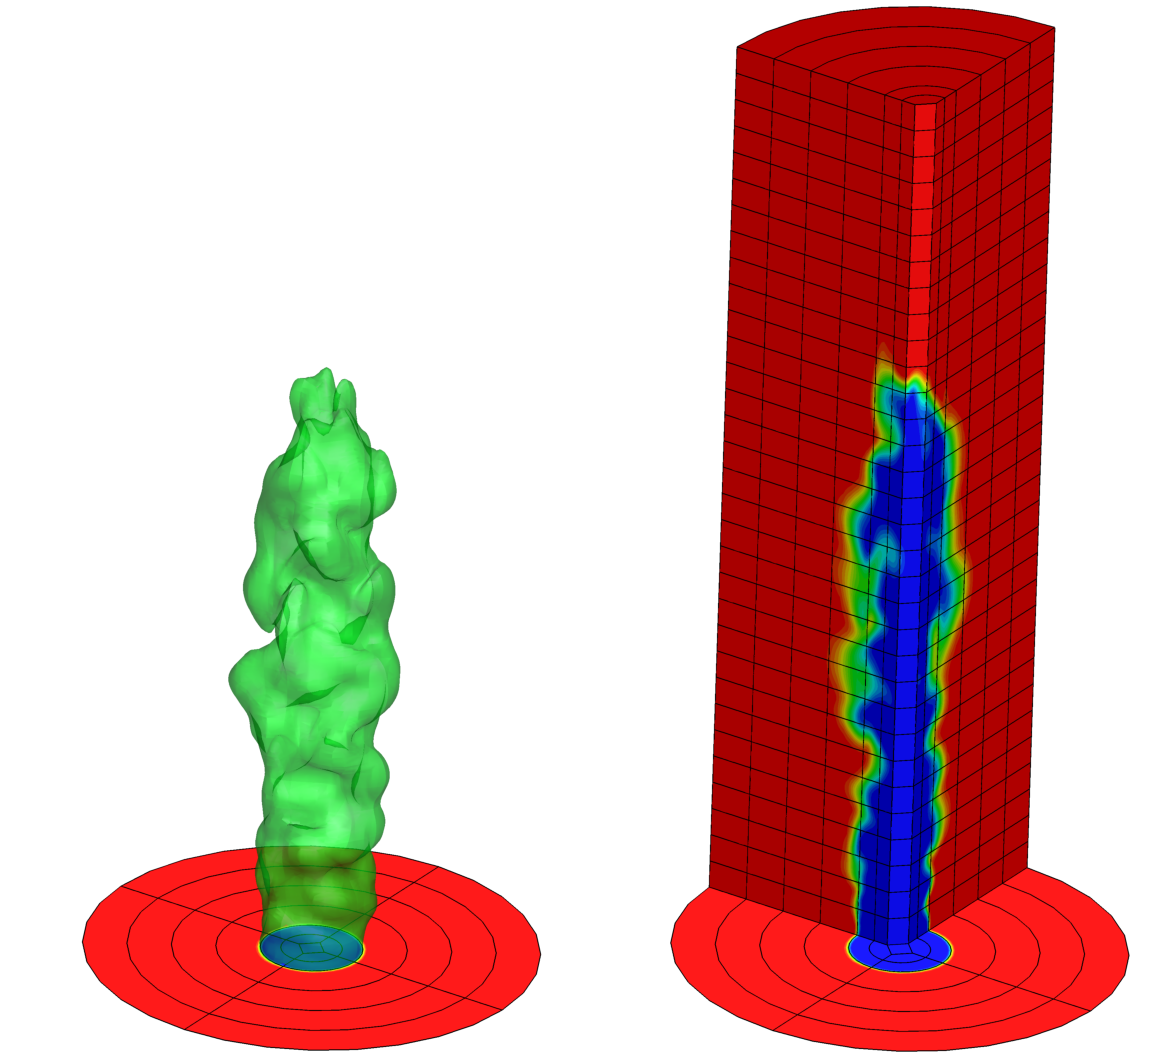
\includegraphics[height=0.25\textwidth]{figs/fsd2_0ms.png}}%
	\:
	\subfigure[At t=4.25ms 5595 (8x8x8) blocks, ~2.8 million cells
(3 levels of mesh refinement)]
   {\label{fig:4msflame}	   
   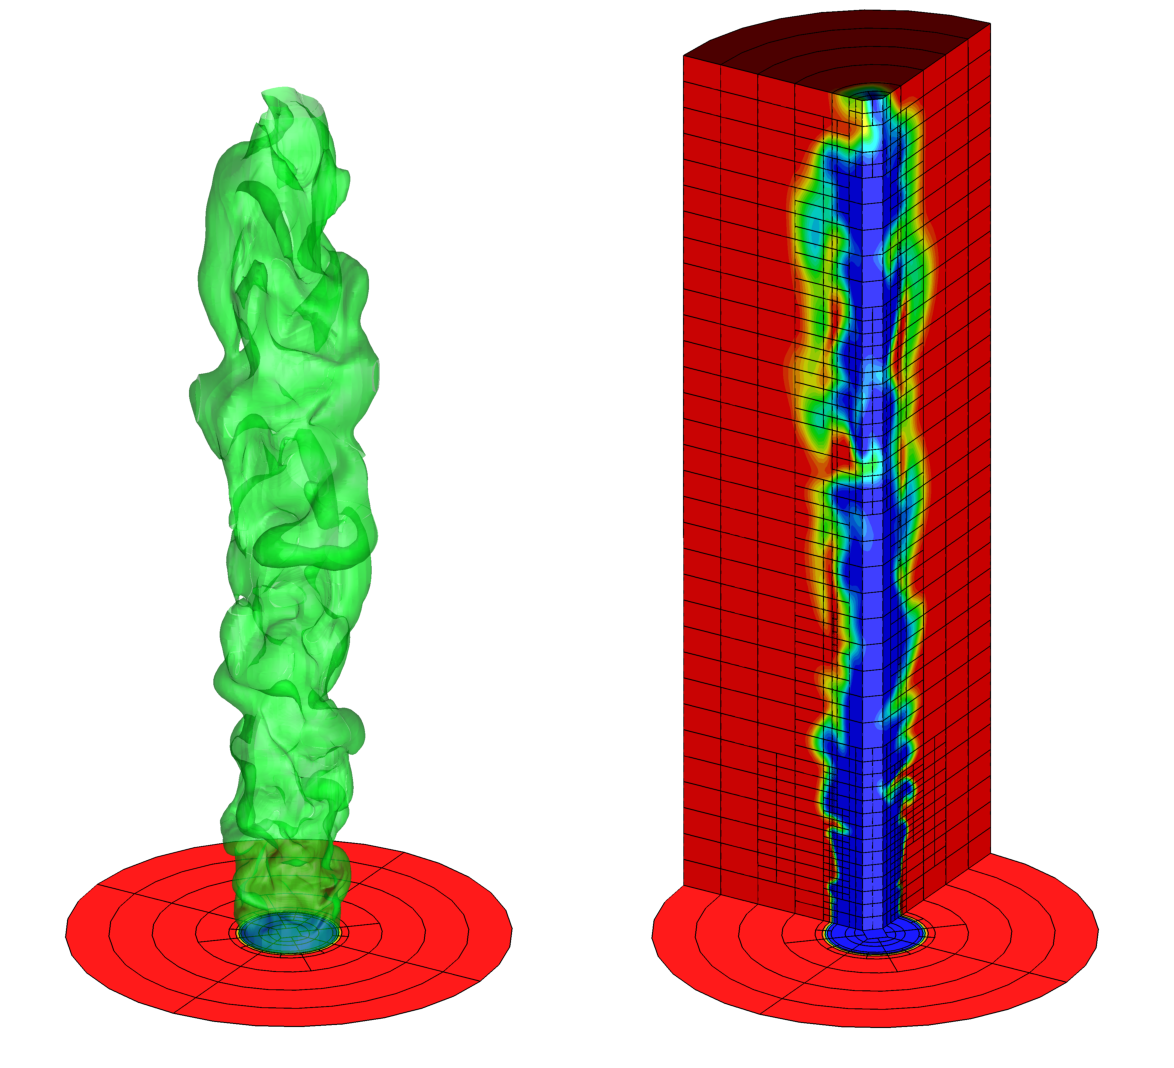
\includegraphics[height=0.25\textwidth]{figs/fsd4_25ms.png}}%
   \:
	\subfigure[At 7.0 ms, 18531 (8x8x8) blocks, ~9.5 million cells
(3 levels of mesh refinement)]
   {\label{fig:7msflame}	   
   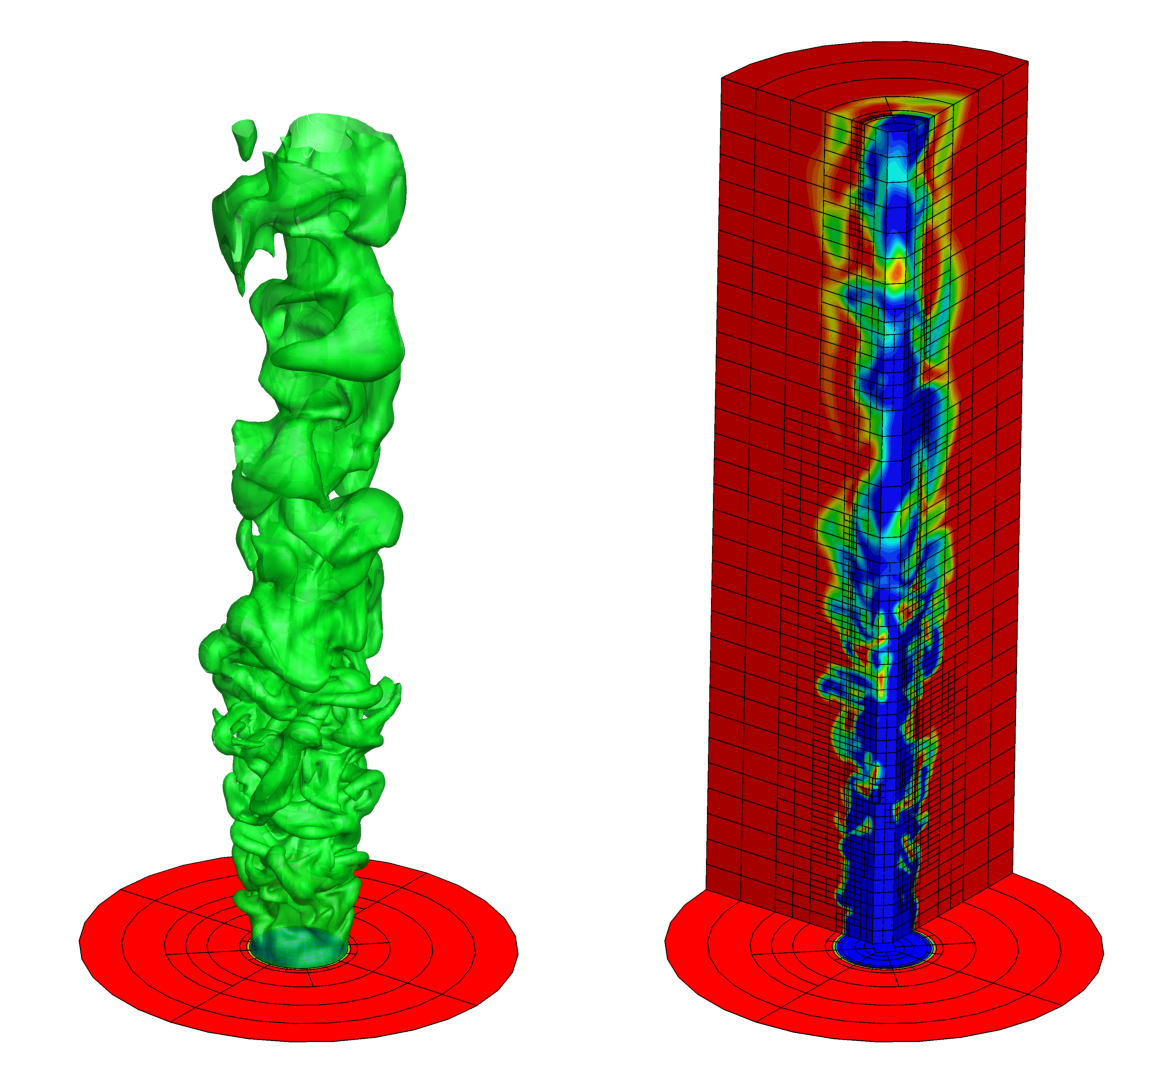
\includegraphics[height=0.25\textwidth]{figs/fsd7_0ms.png}}%
\caption{Some figures showing isotropic mesh refinement with 3 levels of refinement for a lean premixed methane air flame in air. LES solutions were obtained with the flame surface density (FSD) model and the refinement was based on temperature gradient.}   
 \label{fig:LES_case1}        
\end{figure} 

\begin{figure}[t!]
  \centering
	\subfigure[Time averaged $O_2$ species concentration (t = 6-11 ms)]
   {\label{fig:oxygen}	   
  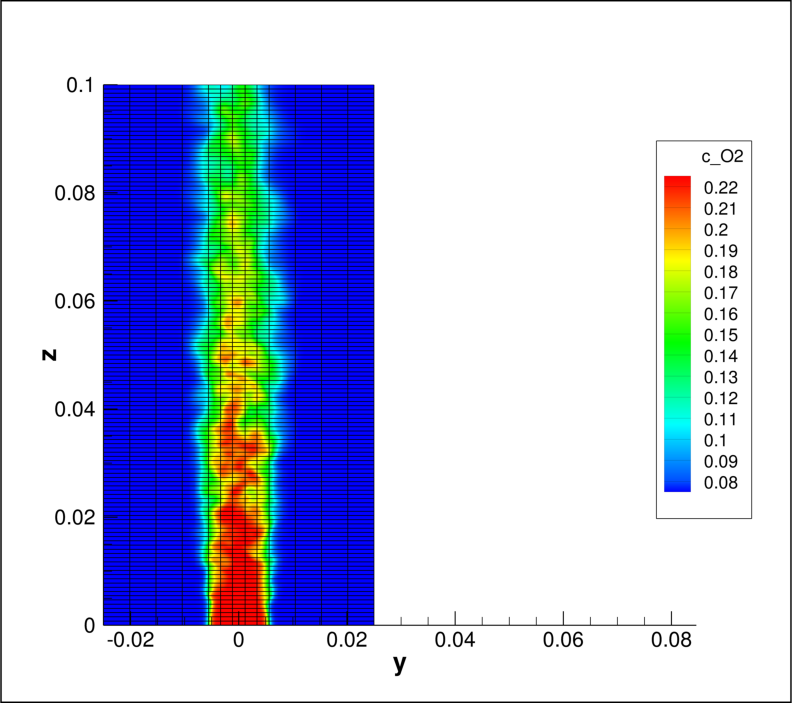
\includegraphics[height=0.4\textwidth]{./figs/Time_averaged_c_O2.png}}%
   \:
  \subfigure[Flame temperature at t= 9.0 ms] 
  {\label{fig:flametemp}
  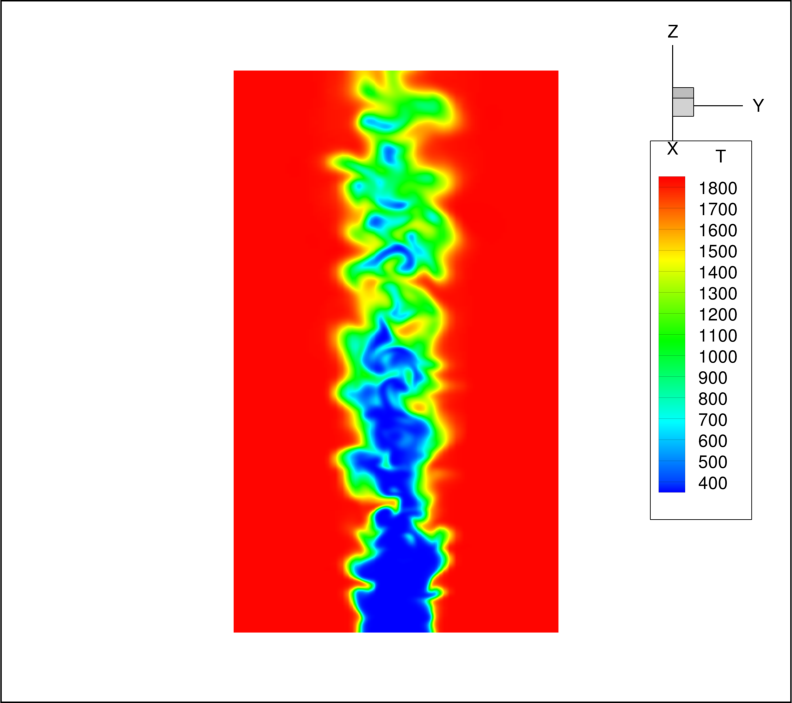
\includegraphics[height=0.4\textwidth]{./figs/Flame_temp.png}}   

\caption{Turbulent premixed methane flame having equivalence ratio $\Phi = 0.7$}    
 \label{fig:LES_case2}        
\end{figure}  


The CFFC code was used to run a simulation for a turbulent premixed methane flame, using 800 nodes, 3200 blocks and each block having $8^3 = 512$ cells, hence a total of $1,638,400$ cells. Time averaged results for t=6ms, 7ms, 8ms, 9ms, 10ms and 11ms are shown in figure~\ref{fig:oxygen}, the contours representing the species concentration of Oxygen.\par


Included here are some pictures from previous CFFC simulations that show the varying mesh cell sizes among the different blocks.

